% --- Gasbot / Sensing configuration ----
\begin{figure}[ht!]
	\begin{center}	
		\vspace{2em}	
		% --- Gasbot ---
		\subfigure[A gas-sensitive mobile robot]{\label{fig:gasbot}		
		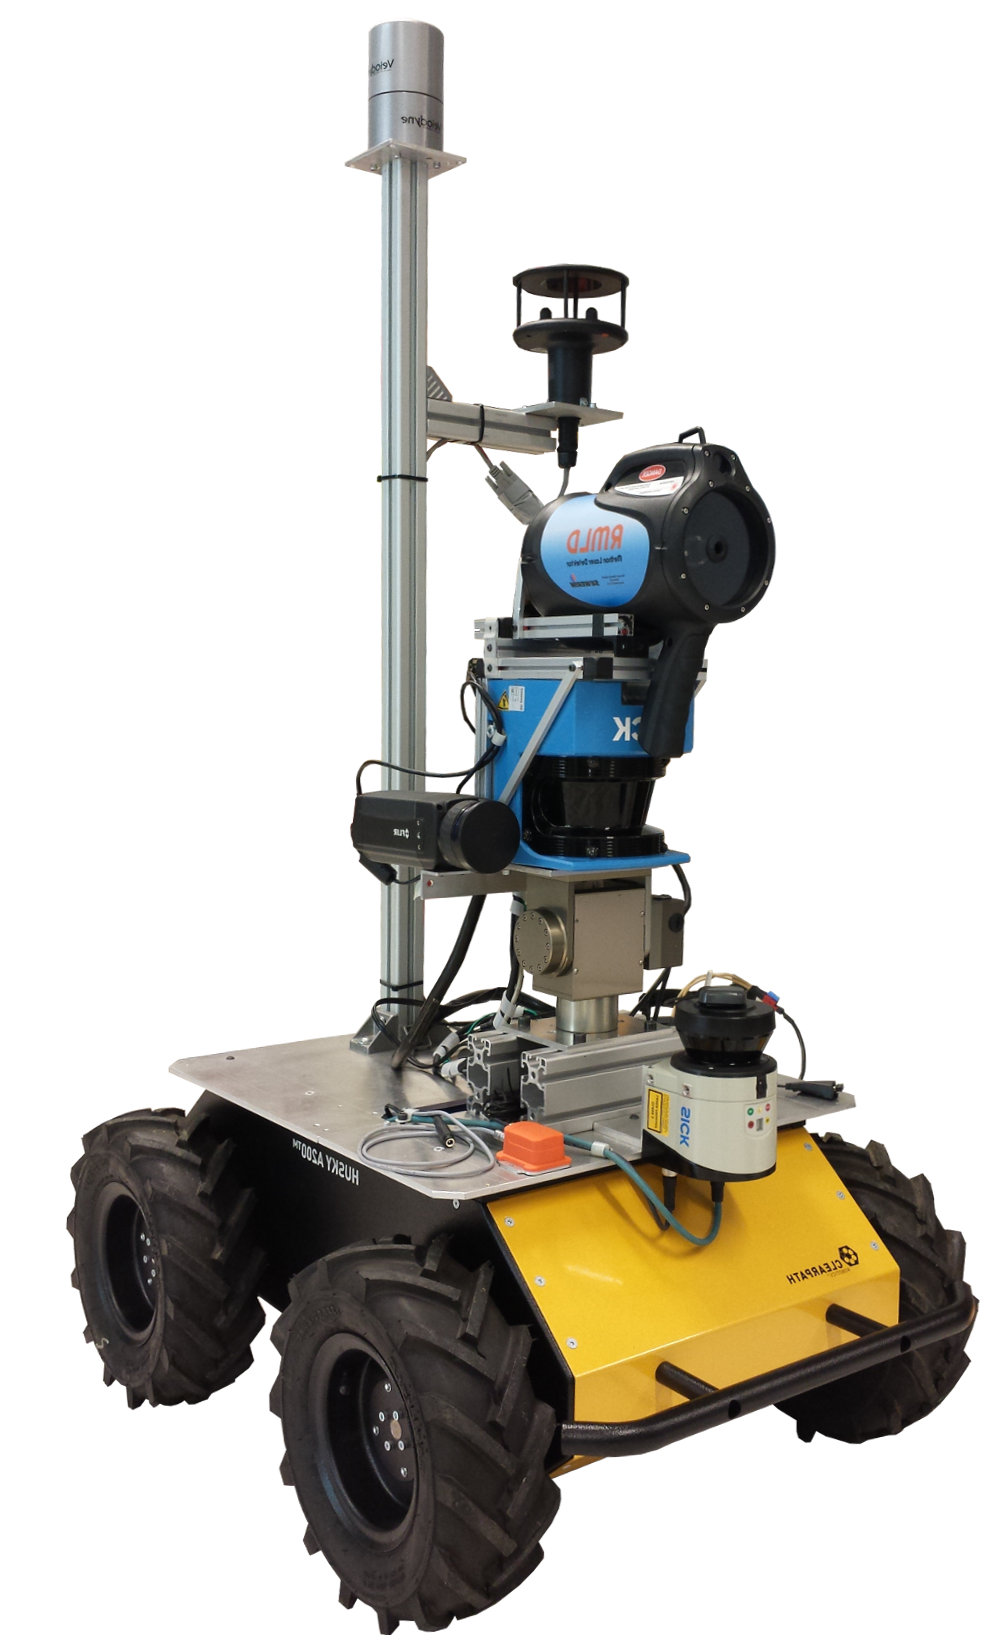
\includegraphics[width=2.5cm]{fig/gasbot.png}}
		% --- TDLAS measurement ---
		\begin{picture}(0,0)
		\put(118,-178){
			\put(-135,230){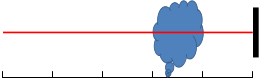
\includegraphics[width=5cm]{fig/RMLD_WorkingPrinciple.png}}
			\small
			\put(-127,272){\FramedBox{0.5cm}{2.5cm}{\textcolor{red}{\small 1200 ppm $\times$ m}}}
			\put(-127,305){\cfbox{white}{\rotatebox{0}{{\tabular[t]{@{}c@{}}Background \\concentration: \\ 200 ppm $\times$ m \endtabular}}}}		
			\put(-060,305){\cfbox{white}{\rotatebox{0}{{\tabular[t]{@{}c@{}}Gas source \\concentration: \\1000 ppm $\times$ m \endtabular}}}}
			\put(-135,220){0}
			\put(-108,220){1}
			\put(-081,220){2}
			\put(-054,220){3}
			\put(-027,220){4}
			\put( 002,220){5 m}}
		\end{picture}
		\hspace{15em}
		% --- Sensing Conf ---
		\subfigure[Sensing configuration]{\label{fig:conf}
		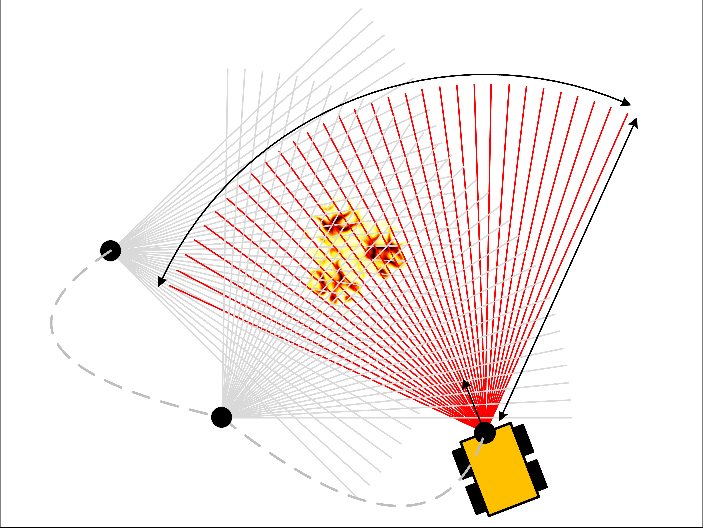
\includegraphics[trim={5 5 5 5}, clip,width=6cm,angle=0,origin=c]{fig/gas_tomography.pdf}}
		\begin{picture}(0,0)
		\normalsize
		\put(60,10){
			\put(-090,050){$r$}
			%\put(-165,008){$<x,y,\theta>$}
			\put(-155,008){$(x,y,\theta)$}
			\put(-160,095){$\phi$}
			\put(-222,055){$c_1$}
			\put(-192,008){$c_2$}
			\put(-102,009){$c_3$}}
		\end{picture}
		\caption{ 
		(a) The robot is equipped with an actuated TDLAS sensor, which reports integral concentration of methane along its line-of-sight.
		(b) A sensing configuration $c$ is sampling a circular sector ($r,\phi$) by emitting $s$ optical beams at pose $(x,y,\theta)$.
		}
	\end{center}
	%\vspace{-2em}
\end{figure}

